%%%%%%%%%%%%%%%%%%%%%%%%%%%%%%%%%
%
%       EXERCÍCIO
%
%%%%%%%%%%%%%%%%%%%%%%%%%%%%%%%%%

\definevalorquestao

\begin{exercicioBanco}[\valorquestao]
A figura mostra um esboço do gráfico da função \(f(x) = a^x + b\), com \(a\) e \(b\) reais, \(a > 0\), \(a \neq 1\) e \(b \neq 0\). Então, o valor de \(f(2) - f(1)\) é igual a:

\begin{center}
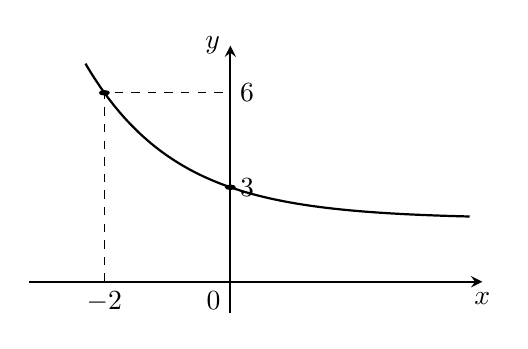
\begin{tikzpicture}[xscale=0.8, yscale=0.4, >=stealth]
    % Eixos cartesianos
    \draw[->, thick] (-3.2,0) -- (4,0) node[below] {$x$};
    \draw[->, thick] (0,-1) -- (0,7.5) node[left] {$y$};
    \node[below left] at (0,0) {$0$};

    % Curva exponencial f(x) = (0.5)^x + 2
    \draw[thick, domain=-2.3:3.8, samples=100] plot (\x, {2 + (0.5)^(\x)});

    % Projeções e marcadores
    \draw[dashed] (-2,0) -- (-2,6) -- (0,6);
    \node[below] at (-2,0) {$-2$};
    \node[right] at (0,6) {$6$};
    \node[right] at (0,3) {$3$};

    \fill (-2,6) circle (2.5pt);
    \fill (0,3) circle (2.5pt);
\end{tikzpicture}
\end{center}

% Define as alternativas
\newcommand{\alternativas}{%
    \begin{center}
        \begin{tabularx}{\textwidth}{XXXXX}
            (a) \(-\dfrac{3}{4}\). &
            (b) \(-\dfrac{15}{4}\). &
            (c) \(-\dfrac{1}{4}\). &
            (d) \(-\dfrac{7}{6}\). &
            (e) \(-\dfrac{35}{6}\).
        \end{tabularx}
    \end{center}
}

% Define a resposta correta
\newcommand{\resposta}{C}

% Lógica condicional para exibição
\ifdefstring{\atividade}{lista}{%
    \alternativas
    \vspace{0.5em}
    
    \noindent\textbf{Resposta:} letra \textbf{\resposta}.
}{%
    \ifdefstring{\modo}{objetivo}{%
        \alternativas
    }{%
        % modo = discursiva → não mostra alternativas
    }
}
\end{exercicioBanco}

